\documentclass{article}
%\usepackage[margin=1in]{geometry}
\usepackage{graphicx} % Required for inserting images
\usepackage{hyperref}
\usepackage{amsmath}
\usepackage{titling}
\usepackage{enumitem}
\usepackage{makecell}
\usepackage{minted}
 \usepackage{url}
\renewcommand\maketitlehooka{\null\mbox{}\vfill}
\renewcommand\maketitlehookd{\vfill\null}

\begin{document}
\title{\Huge Intro ML Homework 6}

\author{ \huge
Jaskin Kabir \\
\Large Student Id: 801186717 \\
\Large \href{https://github.com/jaskinkabir/Intro_ML/tree/main/HM6}{GitHub:}\\\url{https://github.com/jaskinkabir/Intro_ML/tree/main/HM6}
}

\date{November 2024}

\begin{titlingpage}
\maketitle
\end{titlingpage}

\section{Problem 1: Convolutional Neural Networks}
\begin{enumerate}[label=\alph*. ]
    \item \textit{2 Convolutional Layers}
     A convolutional neural network was constructed with 32 filters in the first layer and 64 filters in the second layer. The kernel size was set to 3x3 for both layers. After 200 epochs of training on the CIFAR-10 dataset, the model reached a validation accuracy of 73.8\%, and validation loss curves can be seen in Figure \ref{fig:conv_loss_a}. As can be seen in the graph, there was significant overfitting in the model.
     
     The best performing fully connected model from Homework 6 reached a validation accuracy of 47.2\%, which is 36\% lower than even this two layer convolutional model's accuracy. This demonstrates how much more effective convolutional models are at processing images than fully connected models alone. 
     
     Performance is not the only advantage of convolutional models though. The fully connected model had a total of 985,226 parameters, while the convolutional model had only 150,826. This is a reduction of 85\% in the number of parameters, which is a significant reduction in complexity. This reduction in complexity allows the convolutional model to be trained much faster than the fully connected model. 
     
     The convolutional model finished its 200 epochs of training in only 463 seconds, which is a massive speedup when compared to the 23 minutes it took to train the fully connected model. However, the convolutional model was trained on an Nvidia A100 GPU, whereas the fully connected model was trained on an Nvidia RTX 3070 GPU. This means that the majority of the speedup is due to the difference in hardware, rather than the difference in model complexity.

     \begin{figure}[ht]
        \centering
        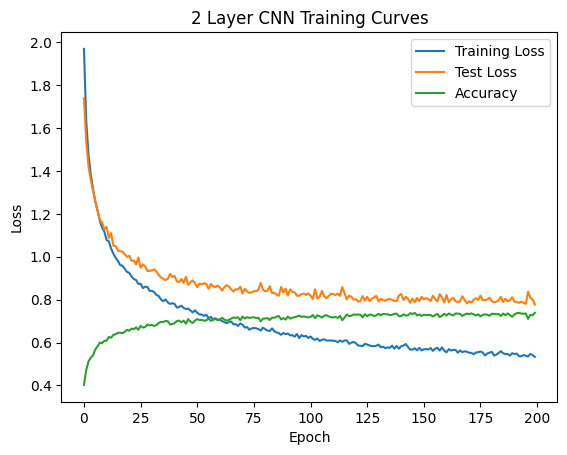
\includegraphics[width=0.55\textwidth]{output/graph1_a.png}
        \caption{Validation loss and accuracy curves for the two layer convolutional model.}
        \label{fig:conv_loss_a}
    \end{figure}
     
     \item \textit{3 Convolutional Layers}
     Adding a third convolutional layer to this model significantly increased the model's propensity to overfit. To handle this issue, lower learning rate and larger weight decay parameters were passed to the model's optimizer. After 200 epochs of training, the model reached a validation accuracy of 73.2\%, which is the same as the two layer model. The validation loss curves for this model can be seen in Figure \ref{fig:conv_loss_b}.

     This model had a total of 159,146 parameters, which is an increase of 5.5\% over the two layer model. The time it took to train this model was 495 seconds, which is 7\% longer than the two layer model. This shows that the training time is not a linear function of the number of parameters. It is possible that a larger model requires more time to load into the GPU's memory, which could explain the discrepancy in training times.

\end{enumerate}
\section{Problem 2: Residual Networks}
A residual network with 10 residual blocks was constructed and trained on the CIFAR-10 dataset. Each residual block consists of two convolutions and batch normalizations, with a dropout layer before the skip connection. Before the residual blocks was two convolutional layers, and there was a dropout layer followed by two fully connected layers after the residual blocks. This deep network had a total parameter count of , which is significantly larger than the two convolutional networks discussed above. After 200 epochs of training, the model reached a validation accuracy of 74.2\%. The loss and accuracy curves for this model can be seen in Figure \ref{fig:res_loss}.

While this model is much more complex than the fully connected network, its skip connections allow the model to be trained much faster. This is why it only took 600 seconds to train the model. The training time was only 30\% longer than the 3 layer convolutional model, which is much less of a difference than the 10x increase in model complexity. The accuracy of the residual network was also \% higher than the 3 layer convolutional model.
\end{document}